\section{Resultados}

\subsection{Función de transferencia de las redes}

Una manera útil de pensar a una red es con un punto de vista basado en teoría de control, a partir del cual construimos una función de transferencia calculando la respuesta de la red a ciertas frecuencias. Así se pueden ver las frecuencias a las que la red tiene mayor o menor sensibilidad.

\begin{figure}[h!]
    \centering
    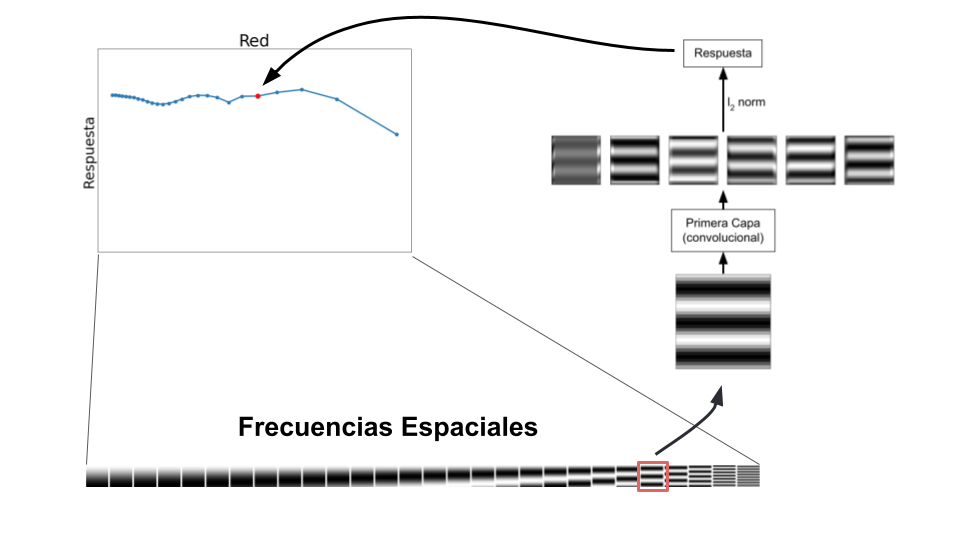
\includegraphics[width=\textwidth, trim={0 2cm 0 0},clip]{images/bode_diagrams/explanation_bode.png}
    \caption{Diagrama de cómo se construye la función de transferencia para cierta red. Primero se generan varias frecuencias en una sola dirección (en este caso vertical) y se ingresan a la primera capa de la red. A la salida de la capa previa a la función de activación se le toma la norma $L_2$, y esa es la respuesta de la red (un escalar) para tal frecuencia.}
    \label{bode_explain}
\end{figure}

\begin{figure}[h!]
    \centering
    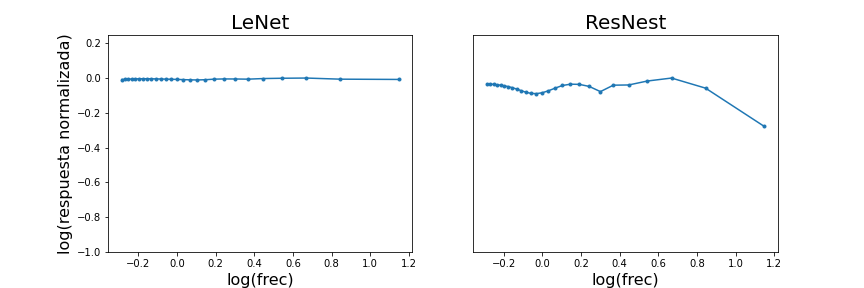
\includegraphics[width=\textwidth]{images/bode_diagrams/mnist_nets.png}
    \caption{Funciones de transferencia para LeNet y ResNet. Las dos son más o menos igual de susceptibles a todas las frecuencias presentadas, pero ResNet sí tiene un poco de modulación negativa con cierta persistencia en las frecuencias altas y para calidades de JPEG intermedias.}
    \label{bode_examples}
\end{figure}



\subsection{¿Qué hace la defensa de JPEG?}

Como vimos en la sección de compresión JPEG, cuando esta es aplicada a una imagen que ha sido sometida a un ataque adversario, los componentes de alta frecuencia se eliminan y, así como los humanos percibimos en menor medida dichos componentes, es posible que la red no logre distinguir el ataque perpetrado sobre la imagen, esto debido a que los ataques suelen tratarse de pequeñas cantidades de ruido o distorsión introducidos en la imagen y, al reducir la calidad de la misma, la red tiene más probabilidades de recuperar la clasificación original de la imagen. Esto se encuentra esquematizado en la Figura \ref{jpegexample}.

\begin{figure}[h!]
    \centering
    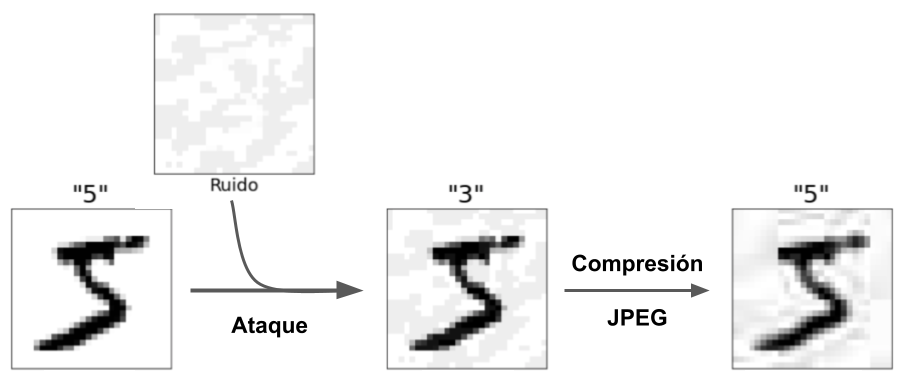
\includegraphics[width=0.8\textwidth]{images/jpeg/jpegdefense_example.png}
    \caption{La defensa JPEG radica en contrarrestar el ruido agregado por el ataque adversario al remover los componentes de alta frecuencia, que son los causantes de la falla en la clasificación de la red. En este ejemplo, el dígito 5 es clasificado como un 3 con el ruido del ataque, pero al hacer una compresión JPEG, la red clasifica correctamente al dígito como un 5.}
    \label{jpegexample}
\end{figure}

En la Figura \ref{jpeg_def} se muestra el resultado de nuestro entrenamiento de las redes LeNet y ResNet utilizando MNIST y el ataque FGSM con la norma $L_\infty$ para distintos niveles de compresión JPEG como defensa. Se observa que, efectivamente, conforme aumenta la compresión (disminuye la calidad), la precisión (accuracy) en la clasificación de las imágenes por parte de la red es mayor. Nótese que con ResNet la precisión decae más rápidamente conforme aumenta el épsilon.
\begin{figure}[h!]
    \centering
    \begin{subfigure}[b]{0.49\textwidth}
        \centering
        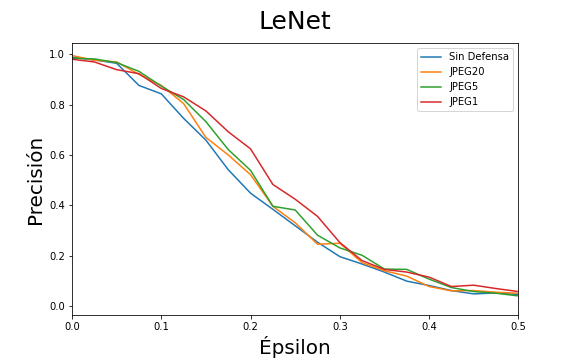
\includegraphics[width=\textwidth]{images/jpeg/jpegdefense_vs_epsilon_linear.png}
        \caption{Compresión JPEG contra FGSM usando LeNet}
    \end{subfigure}
    \begin{subfigure}[b]{0.49\textwidth}
        \centering
        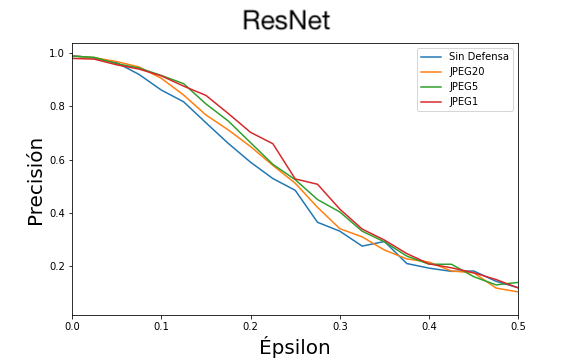
\includegraphics[width=\textwidth]{images/jpeg/jpegdefense_vs_epsilon_nonlinear.png}
        \caption{Compresión JPEG contra FGSM usando ResNet}
    \end{subfigure}
    \caption{Resultado de la compresión JPEG como defensa ante el ataque FGSM sobre MNIST}
    \label{jpeg_def}
\end{figure}

En la Figura \ref{bode_gifs} se observa cómo cambian las funciones de transferencia de cada red cuando las imágenes pasan por distintos niveles de compresión JPEG según el siguiente esquema:
\begin{center}
    frecuencia $\to$ compresión JPEG $\to$ $1^\text{er}$ capa (convolucional) $\to$ respuesta
\end{center}
Se nota que no hay mucho cambio en LeNet para ninguna calidad de compresión. Con respecto a ResNet, sí hay modulación con algunas calidades bajas, más o menos en el rango de 7 a 16, pero no se observa un gran cambio en el desempeño de la red. Cabe mencionar que las calidades más bajas ($1-5$) destruyeron completamente cada frecuencia que pasamos por la red, y por eso no hay ningún cambio en la función de transferencia para esas calidades. Pensamos que eso es un artefacto del tamaño de las imágenes y no se debe tomar al pie de la letra. Asimismo, por el tamaño de las imágenes, hay baja resolución frecuencial, y eso también puede afectar los resultados. Este análisis debe de ser repetido para imágenes más grandes.
\begin{figure}[h]
    \animategraphics[autoplay,loop, width=0.48\linewidth]{5}{images/bode_diagrams/LeNet/}{1}{100}
    \animategraphics[autoplay,loop, width=0.48\linewidth]{5}{images/bode_diagrams/ResNet/}{1}{100}
    \caption{Estos GIFs fueron hechos de la misma manera que la Figura \ref{bode_examples}, pero las frecuencias fueron comprimidas con JPEG antes de pasarlas por la red.}
    \label{bode_gifs}
\end{figure}



\subsection{JPEG en CIFAR-10}

Utilizando LeNet, con los ataques FGSM (Figura \ref{frog_cat_fgsm}), que tiene norma $L_\infty$, y FGM (Figura \ref{frog_cat_fgm}), que tiene norma $L_2$, se tiene una clasificación errónea de la imagen \texttt{train[0]} del conjunto CIFAR-10 a partir del épsilon indicado en la figura. Como en el FGSM cada pixel tiene una mayor intensidad, no se requiere un épsilon tan grande como el de FGM. En la Figura \ref{cifar_accuracy_epsilon} se observa la eficacia de la defensa JPEG contra el ataque FGSM para distintas calidades de la imagen: mientras menor es la calidad, mayor es la precisión de la red al clasificar la imagen. Nótese que hay una desventaja en usar JPEG porque disminuye la precisión de la red entre más baja sea la calidad (Figura \ref{cifar_jpeg_accuracy}).

En la Figura \ref{frog_ruidos} se muestran las transformadas rápidas de Fourier (FFTs) en 2D de los ruidos generados por el FGSM y el FGM, y se observa que ambas FFTs son muy similares a pesar de que los ruidos parecen distintos por la capa gris del FGM. Esto se debe a que, con FGM, los valores de la intensidad del ruido están en el intervalo $(-1, 1)$, pero en FGSM solo pueden ser $-1$ o $1$, entonces los colores son de menor intensidad en FGM: el gris en RGB es $(r,g,b)$ cuando $r \approx g \approx b < 1$.

\begin{figure}[h!]
    \centering
    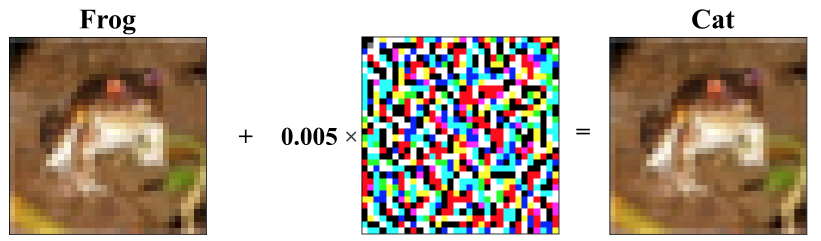
\includegraphics[width=0.80\textwidth]{images/cifar-10/frog_cat_fgsm.png}
    \caption{FGSM sobre CIFAR-10}
    \label{frog_cat_fgsm}
\end{figure}

\begin{figure}[h!]
    \centering
    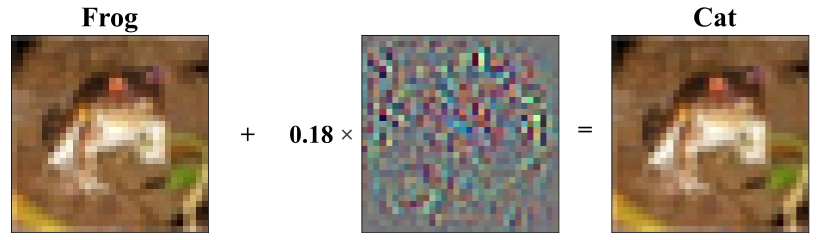
\includegraphics[width=0.81\textwidth]{images/cifar-10/frog_cat_fgm.png}
    \caption{FGM sobre CIFAR-10}
    \label{frog_cat_fgm}
\end{figure}

\begin{figure}[h!]
    \centering
    \begin{subfigure}[b]{0.45\textwidth}
        \centering
        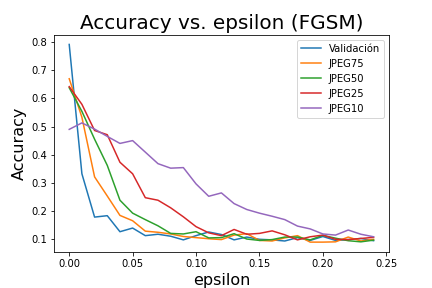
\includegraphics[width=\textwidth]{images/cifar-10/cifar_epsilon_accuracy.png}
        \caption{Precisión de LeNet para distintos valores de la calidad de la imagen en la compresión JPEG}
        \label{cifar_accuracy_epsilon}
    \end{subfigure}
    \hspace{4mm}
    \begin{subfigure}[b]{0.45\textwidth}
        \centering
        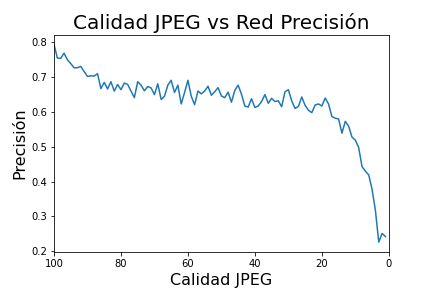
\includegraphics[width=\textwidth]{images/cifar-10/cifar_JPEG_accuracy.png}
        \caption{Precisión de LeNet en función de la calidad de la imagen en la compresión JPEG}
        \label{cifar_jpeg_accuracy}
    \end{subfigure}
    \caption{Eficacia de JPEG}
    \label{cifar_accuracy}
\end{figure}

En la Figura \ref{frog_cat_fft} se muestra cómo la FFT de la imagen original y la imagen atacada parecen exactamente iguales debido a que entre más pixeles y más compleja sea la imagen, la adición del ruido es más sutil, además de que el valor mínimo del épsilon adversario es menor con las imágenes de color. En cambio, con MNIST la adición del ruido sí es observable en la FFT (Figura \ref{fft_mnist}).

\begin{figure}[h!]
    \centering
    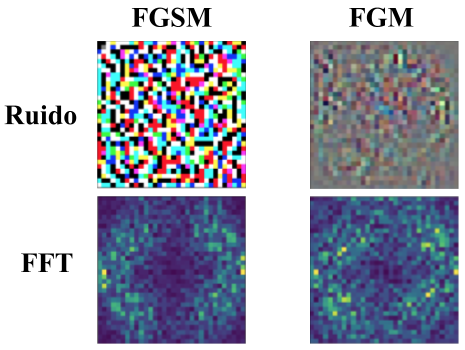
\includegraphics[width=0.5\textwidth]{images/cifar-10/frog_noises.png}
    \caption{La FFT de los ruidos de FGSM y FGM}
    \label{frog_ruidos}
\end{figure}

\begin{figure}[h!]
    \centering
    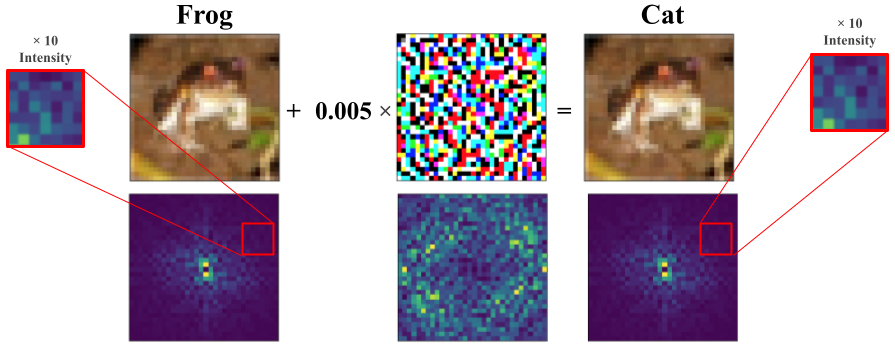
\includegraphics[width=\textwidth]{images/cifar-10/frog_cat_fgsm_fft.png}
    \caption{Comparación de la FFT de la imagen original y de la imagen con el ruido agregado por FGSM}
    \label{frog_cat_fft}
\end{figure}

\begin{figure}[h!]
    \centering
    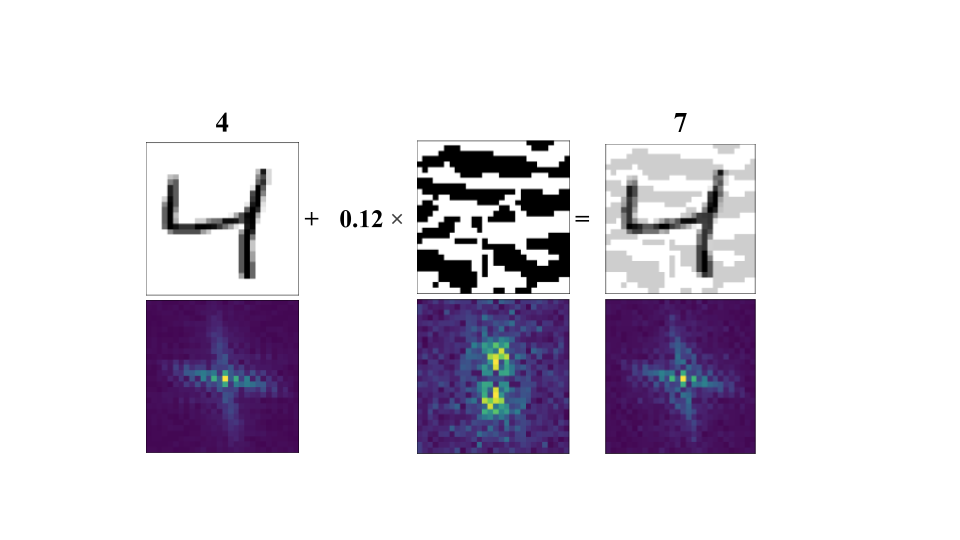
\includegraphics[width=0.65\textwidth]{images/mnist/ffts.png}
    \caption{Con MNIST sí se observa una pequeña contribución del ruido en la FFT de la imagen adversaria.}
    \label{fft_mnist}
\end{figure}

\pagebreak

\subsection{Los efectos de overfitting y overparameterization}

Se ha sugerido que algunas propiedades de ciertas redes pueden contribuir a su susceptibilidad a los ataques adversarios. Por ejemplo, en el contexto de las imágenes médicas y sus respectivas redes, se propone que el sobreajuste (overfitting) y la sobreparametrización (overparameterization) pueden actuar de esa manera \cite{ma2020understanding}. El \textit{overfitting} ocurre cuando el modelo clasifica bien los datos de entrenamiento, pero no se generaliza tan bien, es decir, en los datos de validación tiene peor desempeño. La \textit{overparameterization} tiene lugar cuando hay tantos parámetros que la red es capaz de ``memorizar'' completamente los datos. Hicimos un pequeño análisis para probar esta hipótesis y no encontramos resultados que la apoyen. De hecho, con las redes que probamos, encontramos lo opuesto. En general, el overfitting y la overparameterization hacen que la red sea más robusta a los ataques adversarios (Figure \ref{overaparam_overfit}).

Para explorar el overfitting, la red LeNet fue modificada al ser entrenada con 5 cantidades distintas de épocas (epochs). Mientras más épocas, mayor es la probabilidad de que la red haya sido sobreajustada (overfit). Para explorar la overparameterization, la red fue entrenada con distintas cantidades de parámetros, agregando un cierto número de capas (layers) adicionales directamente antes de la última, cada capa adicional con 256 nodos (Tabla \ref{overparam_table}).

\renewcommand{\tablename}{Tabla}
\begin{table}[h!]
    \centering
    \begin{tabular}{|c|c|}
     \hline
     Red & Número de parámetros  \\ 
     \hline
     Normal & $61,706$  \\ 
     \hline
     2 Capas Adicionales & $150,978$  \\ 
     \hline
     4 Capas Adicionales & $282,562$  \\ 
     \hline
     6 Capas Adicionales & $414,146$  \\ 
     \hline
     10 Capas Adicionales & $743,106$  \\ 
     \hline
     20 Capas Adicionales & $1,335,234$  \\ 
     \hline
    \end{tabular}
    \caption{Número de parámetros con cada conjunto de capas adicionales en la red LeNet.}
    \label{overparam_table}
\end{table}

\begin{figure}[h!]
    \centering
    \begin{subfigure}[b]{0.49\textwidth}
        \centering
        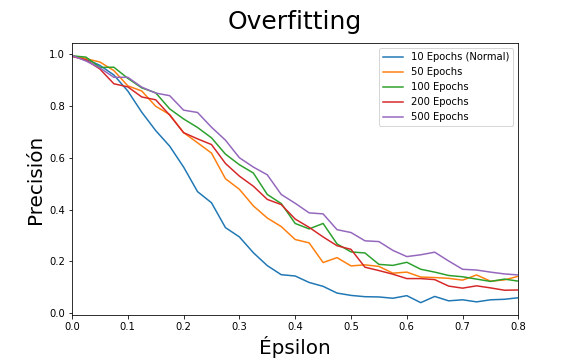
\includegraphics[width=\textwidth]{images/overfit_vs_attack.png}
        \caption{Overfitting en LeNet}
        \label{overfit}
    \end{subfigure}
    \begin{subfigure}[b]{0.49\textwidth}
        \centering
        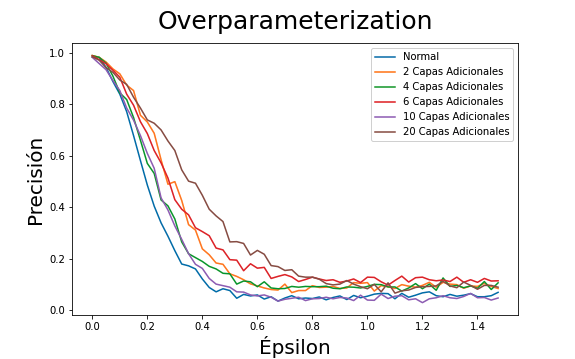
\includegraphics[width=\textwidth]{images/overparam_vs_attack.png}
        \caption{Overparameterization en LeNet}
        \label{overparam}
    \end{subfigure}
    \caption{a) El overfitting consiste en tener exceso de épocas. Aquí se observa que conforme aumenta el número de épocas, la precisión aumenta con respecto a cada épsilon. b) La overparameterization consiste en exceso de capas. En general, aumentar el número de capas aumenta la precisión.}
    \label{overaparam_overfit}
\end{figure}

\pagebreak
    
\subsection{Saliency}
La puntuación (score) $S(I)$ de una imagen es la salida de la capa de la red neuronal justo antes de que se convierta en probabilidades (esto sucede en la función de activación softmax). El procedimiento para obtener la prominencia (\textbf{saliency}) de la imagen es el siguiente:

\noindent
Dada una imagen $I_0$ y una clase $c$, sea $S_c(I_0)$ la puntuación de la clase $c$. 

\noindent
Nos gustaría rankear a los pixeles de $I_0$ con base en su influencia sobre la puntuación $S_c(I_0)$.

\noindent
Podemos aproximar $S_c(I)$ con una función lineal en la vecindad de $I_0$ al calcular la expansión de Taylor a primer orden,
\[S_c(I) \approx w^\top I + b,\]
donde $w$ es la derivada de $S_c$ con respecto de la imagen $I$ en el punto (imagen) $I_0$,
\[w = \left. \frac{\partial S_c}{\partial I} \right |_{I_0}.\]

\noindent
La magnitud de la derivada nos indica cuáles son los pixeles que deben ser cambiados en la menor cantidad para afectar la puntuación de la clase en la mayor medida. Así es como se define la prominencia (saliency) \cite{simonyan2014deep}.


\begin{figure}[h!]
    \centering
    \begin{subfigure}[b]{0.47\textwidth}
        \centering
        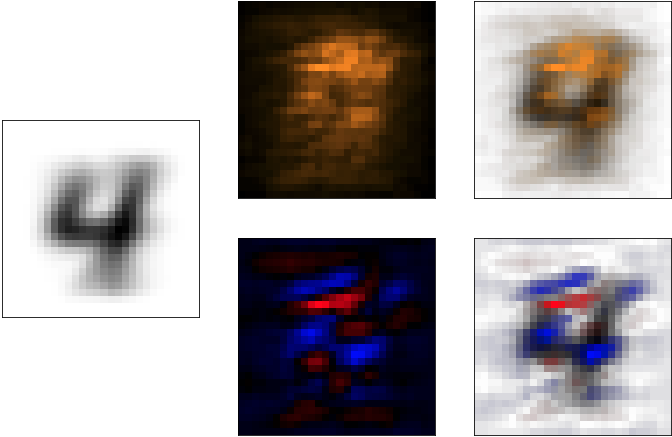
\includegraphics[width=\textwidth]{images/saliency/mnist/linear/4_saliency_figures.png}
        \caption{}
        \label{4_saliency}
    \end{subfigure}
    \hfill
    \begin{subfigure}[b]{0.47\textwidth}
        \centering
        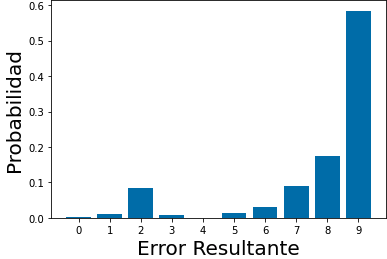
\includegraphics[width=\textwidth]{images/saliency/mnist/linear/4_error.png}
        \caption{}
        \label{4_error}
    \end{subfigure}
    \caption{}
    \label{4_SAL}
\end{figure}

\begin{figure}[h!]
    \centering
    \begin{subfigure}[b]{0.47\textwidth}
        \centering
        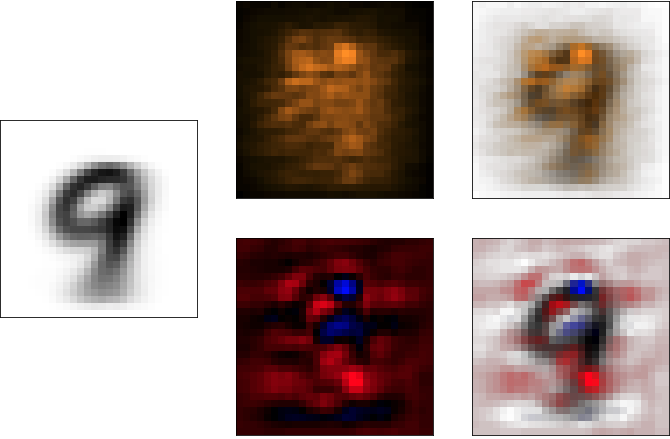
\includegraphics[width=\textwidth]{images/saliency/mnist/linear/9_saliency_figures.png}
        \caption{}
        \label{9_saliency}
    \end{subfigure}
    \hfill
    \begin{subfigure}[b]{0.47\textwidth}
        \centering
        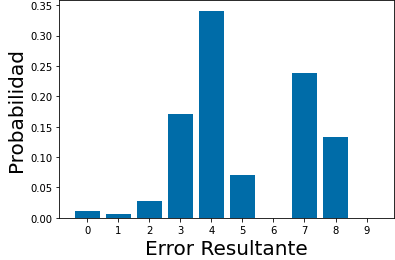
\includegraphics[width=\textwidth]{images/saliency/mnist/linear/9_error.png}
        \caption{}
        \label{9_error}
    \end{subfigure}
    \caption{}
    \label{9_SAL}
\end{figure}

\begin{figure}[h!]
    \centering
    \begin{subfigure}[b]{0.47\textwidth}
        \centering
        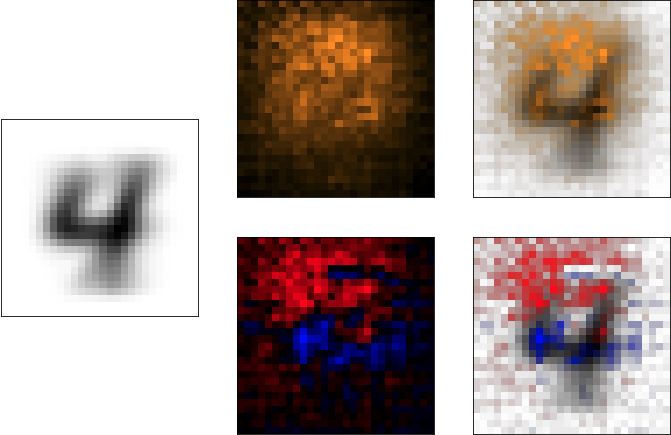
\includegraphics[width=\textwidth]{images/saliency/mnist/nonlinear/4_saliency_figures.png}
        \caption{}
        \label{4_saliency_nonlin}
    \end{subfigure}
    \hfill
    \begin{subfigure}[b]{0.47\textwidth}
        \centering
        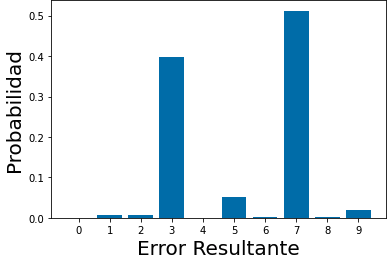
\includegraphics[width=\textwidth]{images/saliency/mnist/nonlinear/4_error.png}
        \caption{}
        \label{4_error_nonlin}
    \end{subfigure}
    \caption{}
    \label{4_SAL_NONLIN}
\end{figure}

\begin{figure}[h!]
    \centering
    \begin{subfigure}[b]{0.47\textwidth}
        \centering
        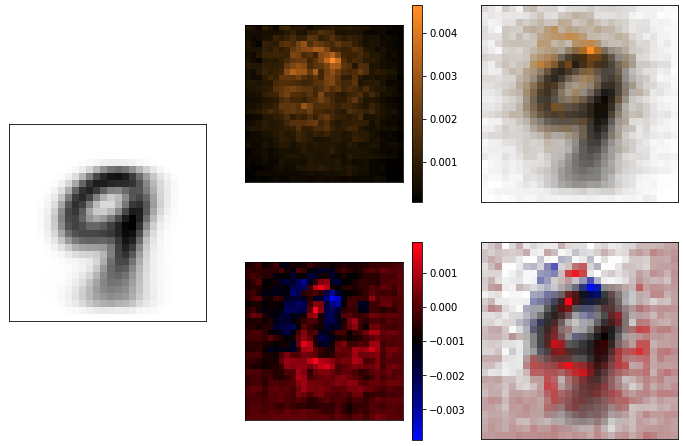
\includegraphics[width=\textwidth]{images/saliency/mnist/nonlinear/9_saliency_figures.png}
        \caption{}
        \label{9_saliency_nonlin}
    \end{subfigure}
    \hfill
    \begin{subfigure}[b]{0.47\textwidth}
        \centering
        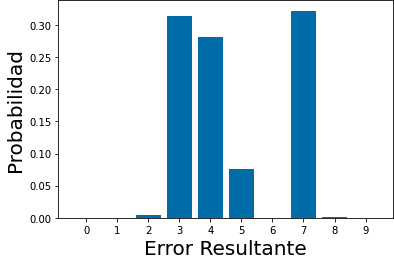
\includegraphics[width=\textwidth]{images/saliency/mnist/nonlinear/9_error.png}
        \caption{}
        \label{9_error_nonlin}
    \end{subfigure}
    \caption{}
    \label{9_SAL_NONLIN}
\end{figure}


\begin{itemize}
    \item Show figures from notebook of how adversarial noise attacks parts of the image that seem vulnerable (for example changing a 3$\to$8)
    \item ``first error'' images for both cifar and mnist
    \item Show Gradient-based localization of both image sets and how they change after adding adversarial noise\cite{Selvaraju_2019}
    \item See the saliency of an attacked image
\end{itemize}